%%%%%%%%%%%%%%%%%%%%%%%%%%%%%%%%%%%%%%%%%
% FRI Data Science_report LaTeX Template
% Version 1.0 (28/1/2020)
% 
% Jure Demšar (jure.demsar@fri.uni-lj.si)
%
% Based on MicromouseSymp article template by:
% Mathias Legrand (legrand.mathias@gmail.com) 
% With extensive modifications by:
% Antonio Valente (antonio.luis.valente@gmail.com)
%
% License:
% CC BY-NC-SA 3.0 (http://creativecommons.org/licenses/by-nc-sa/3.0/)
%
%%%%%%%%%%%%%%%%%%%%%%%%%%%%%%%%%%%%%%%%%


%----------------------------------------------------------------------------------------
%	PACKAGES AND OTHER DOCUMENT CONFIGURATIONS
%----------------------------------------------------------------------------------------
\documentclass[fleqn,moreauthors,10pt]{ds_report}
\usepackage[english]{babel}

\graphicspath{{fig/}}




%----------------------------------------------------------------------------------------
%	ARTICLE INFORMATION
%----------------------------------------------------------------------------------------

% Header
\JournalInfo{FRI Data Science Project Competition 2024}

% Interim or final report
\Archive{Machine Learning report} 
%\Archive{Final report} 

% Article title
\PaperTitle{CnC Counterfactual Visualiser} 

% Authors (student competitors) and their info
\Authors{Cristian Bassotto, Camile Lendering, and Nikolay Kormushev}

% Advisors
\affiliation{\textit{Advisors: prof. dr. Erik Štrumbelj }}

% Keywords
\Keywords{XAI, UX, Counterfactuals}
\newcommand{\keywordname}{Keywords}


%----------------------------------------------------------------------------------------
%	ABSTRACT
%----------------------------------------------------------------------------------------

\Abstract{
Counterfactuals are a crucial tool in explainable AI, offering insights into model decisions by presenting alternative scenarios. While many papers focus on generating counterfactuals, few address visualization. Existing works often feature rudimentary interfaces, rely on specific generators, or lack user validation.

In this paper, we propose a model-agnostic counterfactual UI emphasizing simplicity. We aim for a streamlined user experience, informed by psychology, and validated through a user study. Our goal is to enhance the accessibility and interpretability of counterfactual explanations, advancing explainable AI.
}

%----------------------------------------------------------------------------------------

\begin{document}

% Makes all text pages the same height
\flushbottom 

% Print the title and abstract box
\maketitle 

% Removes page numbering from the first page
\thispagestyle{empty} 

%----------------------------------------------------------------------------------------
%	ARTICLE CONTENTS
%----------------------------------------------------------------------------------------

\section*{Introduction}
Counterfactuals are established as one of the main approaches in explainable AI (XAI). They offer the user insight on how model decisions are made, by providing counterfactual examples of a sample, showing the changes in feature values needed for that sample to be labeled differently. 


There are many papers written that focus on the process of generating counterfactuals with a wide variety of approaches~\cite{keane2020good}, but far less papers that focus on the visualisation aspects. Most visualisation methods found in literature present either underdeveloped or overly complex user interfaces, rely on a specific counterfactual generator or do not validate their method with a user study. This research aims to address these shortcomings by developing a user-friendly, model agnostic counterfactual visualization method.

\subsection*{Related works}
From the counterfactual visualisation methods we looked at, we really liked the approach of SDA-Vis \cite{garcia2022sda} which is a great visualisation and unlike most other papers they did a simple user study. Still we feel can the UI be a bit convoluted and that it is focused in a specific domain. It does have the potential to generalise but we believe it needs some getting used to and is more tailored somewhat more expert users which is not what our goal of simplicity is. 

AdViCE \cite{gomez2021advice} and DECE \cite{cheng2020dece} are two other examples of tools that visualise counterfactuals but are either by design or ended up being not suitable for end users.

Simpler UIs we looked at are ViCE \cite{gomez2020vice} which only works with numeric values and an attempt at an improvement \cite{guyomard2023interactive} which has a similar interface but supports categorical values. The issue we found with their approach is that it does not scale well if we increase the number of features as the interface will start displaying too much information and this becomes less interpretable. The densities of variables used as coloring in ViCE can also be confusing and hard to understand. 

In the visualisation tool proposed by Guyomard et al. \cite{guyomard2023interactive} counterfactuals need to be generated beforehand and input as a json format which makes the solution counterfactual model-agnostic but can require an expert to use. 

An issue with all the UIs we mentioned so far is that they do not take into account psychological aspects. The authors of \cite{warren2022better} argue that based on a study users have an easier time interpreting categorical values compared to continuous numbers so it might be a better idea to divide continuous values into bins or ranges..

\subsection*{Purpose}
Based on our research in our paper we plan to develop a counterfactual model-agnostic UI with a focus on end-users and with as little expert intervention as possible for initial configuration. We want a streamlined user experience that makes the process of generating and understanding counterfactuals as easy as possible. We will work with tabular data containing both continuous and categorical features and we test and improve on the psychological approach suggested in \cite{warren2022better} by using configurable binning and performing a user study to validate the results.
%------------------------------------------------
\section*{Methods}

In this section we outline our methods for developing and evaluating a user-centered, model-agnostic counterfactual explanation visualisation system for tabular data.

\subsection*{Visualisation}
In Figure \ref{fig:main_page}, we have created an initial sketch based on our ideas so far. On the right, the generation procedure and selection of the counterfactual choosen; in the center the comparison between initial instance and final counterfactual prediction and features. Model, dataset and method are selectable in the menu on the left and displayed as title on the top.
\begin{figure}[h]\centering
	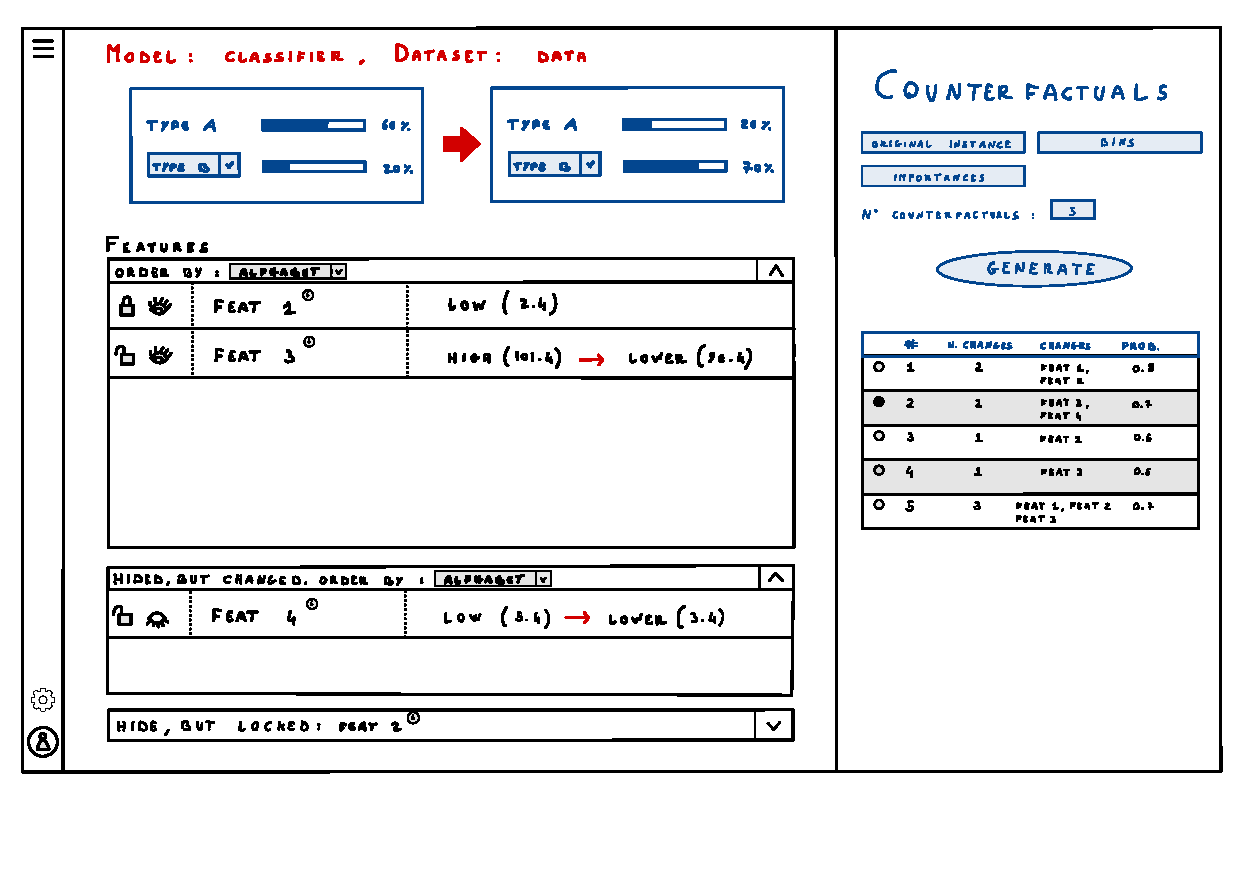
\includegraphics[width=\linewidth]{fig/counterfactual_main.pdf}
	\caption{Initial sketch of the final visualization.}
	\label{fig:main_page}
\end{figure}

\subsection*{Model-agnostic Counterfactual Generation}
A Django back-end is implemented to handle counterfactual generation requests. The back-end accepts \texttt{GET} requests containing an instance in JSON format and returns corresponding counterfactual examples. The system is model-agnostic, meaning that users can  upload their own trained models and datasets for generating counterfactual instances. The only requirement is that the model is differentiable. But, it can be argued that most non-differentiable models (Decision Trees, Rule based systems) are inherently more interpretable.

\subsection*{Model-Agnostic Binning}
To make the counterfactual explanations more interpretable, a model-agnostic binning method will be implemented. This transforms continuous feature values into discrete bins, aligning with the findings of Warren et al.~\cite{warren_et_al_user_study_2023} that show improved user understanding of counterfactual explanations with categorical features. We will use the local transformation method: CAT-CFLocal as described in~\cite{warren2022better}, where continuous feature values in the counterfactual instance are re-labelled as being "higher" or "lower" relative to the values in the original instance. 

%Todo: Compare different binnning techniques.

\subsection*{User Study}
While there exist many numerical evaluation metrics for counterfactual explanations, such as sparsity and proximity~\cite{keane2020good}, these measures are not suitable for evaluating the discretised counterfactual instances. Hence, a user study will be conducted to evaluate the effectiveness our proposed visualization method.

%Todo: Clearly define how the user study will be conducted.



%------------------------------------------------

%\section*{Results}


%------------------------------------------------

%\section*{Discussion}


%------------------------------------------------

%\section*{Acknowledgments}




%----------------------------------------------------------------------------------------
%	REFERENCE LIST
%----------------------------------------------------------------------------------------
\bibliographystyle{unsrt}
\bibliography{report}


\end{document}